\chapter{Methodology}\label{methodology}

In this chapter, we provide a description of the implementation, the employed external software libraries, computational resources, and an environment setup. We outline the datasets, network architecture, training process, and hyperparameter search. A repository containing the source code of our solution along with a Docker container for the training environment are publically available online\footnote{In the attachment \ref{github_main} or online at \url{https://github.com/mpicek/reCNN_visual_prosthesis}} \footnote{In the attachment \ref{docker_image} or online at \url{https://github.com/mpicek/csng_dl_docker_image}}.

\section{Used Software Libraries}

We implemented the solution in a deep learning Python library PyTorch \citep{paszke2019pytorch} with PyTorch Lightning framework\footnote{\url{https://www.pytorchlightning.ai/}} to help us scale the training. NumPy \citep{van2011numpy} and Matplotlib \citep{hunter2007matplotlib} libraries were used for data manipulation and visualization.

\subsection{Nuralpredictors}

The principal component we used to build our solution is the Neuralpredictors library\footnote{\url{https://github.com/sinzlab/neuralpredictors}} developed by Sinz Lab\footnote{\url{https://sinzlab.org/}}, containing the implementation of an extensive amount of neural network layers, regularizations, measure metrics, and other handy utilities designed for neural response prediction primarily in the striate cortex. Many publications related to our problem utilized and extended this library, namely Lurz et al.\citep{lurz2021generalization} who implemented FullGaussian2d readout, and its isotropic three-dimensional version is also present in Neuralpredictors, on which our readout is built upon. Next significant contribution is the reimplementation of rotation-equivariant CNN \citep{ecker2018rotation} from TensorFlow \citep{tensorflow2015-whitepaper} to PyTorch, which we exploited for the core’s construction.

\section{Datasets}

For the DNN training, two distinct datasets were used. The first dataset comes from a publication from Lurz et al. \citep{lurz2021generalization} who measured neural population responses to grayscale images as a visual input in a mouse's primary visual cortex. This dataset was chosen to validate the trained networks to prove that they work correctly.

The most essential dataset for this work, however, is obtained from a computational model developed by Antolík and his colleagues \citep{antolik2019comprehensive}. Being the dataset generated in-silico, the actual locations of the neurons and their preferred orientations are available. We took advantage of this ground truth data to evaluate the precision of neural location and preferred orientation estimates.

As the computational model of the striate cortex can give us virtually unlimited amounts of valuable information, the synthetic dataset is likely to be beneficial for future experiments in this area of research. Using both in-silico and experimental datasets, we can observe differences in the network’s training and examine whether the dataset generated by Antolík et al. model is appropriate for stimulation protocol development.

\subsection{Lurz et al. Dataset - The Mouse Dataset}

The first dataset is a publicly available subset of data from Konstantin-Klemens Lurz and his colleagues' publication \citep{lurz2021generalization}, which we obtained with the authors' consent. The following text will be a paraphrased description of the data. For further details, we refer to the original publication.

The dataset is composed of pairs of visual stimuli and neural population responses. The visual stimuli are cropped grayscale images sampled from ImageNet \citep{deng2009imagenet}, which were upsampled to the resolution of $1080 \times 1920$ and presented at a distance of 15\,cm from the mouse’s head. This dataset contains the images in a resolution of $64 \times 36$px as they were isotropically downsampled, corresponding to a resolution of 0.53\,pixels per degree of visual angle. Although the original data have records from multiple mice, public access is restricted to records from just one subject, whose overall 5335 neurons were recorded from the striate cortex, in particular from layer L2/3. For this purpose, a wide field two-photon microscope \citep{sofroniew2016large} was used along with a genetically encoded calcium indicator GCaMP6s in the recorded mouse. The cells were selected based on a classifier for somata \citep{pnevmatikakis2016simultaneous}. The reported value corresponding to neural activity is an averaged cell’s activity in a certain time window. Data preprocessing and stimulation paradigm were adapted from \citep{walker2019inception}.

The dataset is divided into three subsets. The training set contains 4472 stimulus-response pairs and the validation set 522 pairs. To evaluate our model by measuring the correlation of averaged trials, the test set includes 990 stimulus-response pairs, of which only 99 stimuli were unique, each repeated ten times.

From now on, we will also refer to this dataset as the mouse or experimental dataset.


\subsection{Dataset from Antolík’s Model of V1 - The Synthetic Dataset}

Compared to the first dataset experimentally measured on living mice, this dataset is obtained using a computational model of a cat’s striate cortex developed by Antolík and his colleagues \citep{antolik2019comprehensive}. This in-silico primary visual cortex comprises 65000 neurons modeled as exponential integrate-and-fire point neurons \citep{brette2005adaptive} and divided into three groups: LGN neurons, layer 4 and layer 2/3 (respectively 5000, 30000, and 30000 neurons). The cortical neurons are furthermore divided into populations of excitatory and inhibitory neurons. LGN neurons send connections only to layer 4, and cortical neurons follow specific inter-layer and intra-layer connectivity rules. As regards such rules and the value of other parameters, Antolík et al. model is constrained population of neurons per population by a multitude of experimental findings and data measurements, making both the simulated spontaneous and visually evoked activity reliably close to the behavior of a real cat’s V1. Importantly, orientation maps are also included in the model. From now on, we will refer to this dataset as the synthetic dataset.

Being this dataset produced in-silico, it is not restrained in terms of the number of trials; therefore, compared to the mouse dataset, it is much more voluminous. The pairs of visual stimuli and neural population responses contain resized and cropped grayscale images from ImageNet \citep{deng2009imagenet} of resolution $110 \times 110$\,px and the responses of 30000 neurons from layer L2/3. Responses are obtained by summing the number of spikes within a 500\,ms time window corresponding to stimulus presentation. 

In this dataset, each visual stimulus spans 11 degrees of the visual field. The cortical neurons are, however, distributed in a region of the cortex corresponding to the 4 central degrees of the visual area covered by the stimuli. This was chosen to avoid boundary effects and accommodate the cortical neurons' full receptive field.
The data is divided into three groups of stimulus-response pairs. The training dataset consists of 42250 samples and a validation dataset of 5000 samples. The test set comprises 5000 image-response pairs, of which 500 images are unique, each presented to the model 10 times.

This dataset, however, is not publicly available. To grant access, please, contact us.


\subsection{Pytorch Lightning DataModules}

For a convenient manipulation with the datasets, we implemented a DataModule class from the PyTorch Lightning library for both datasets separately. This facilitates straightforward data handling and its feeding into the neural networks. Our implementation is conducive for future work as it can be easily reused.

\section{Network Architecture}

From a mathematical point of view, this work aims to develop a function generalizable across neurons that, given an image of resolution $H \times W$, receptive field positions, and preferred orientations of $m$ cortical neurons, returns a prediction of the neural population response. That is:

\begin{equation}
f: (\mathbb{R}^{H \times W \times 1} \times \mathbb{R}^m  \times  \mathbb{R}^m  \times  \mathbb{R}^m) \to \mathbb{R}^m,
\end{equation}

where the first parameter is the grayscale input image of resolution $H \times W$, the next two parameters are the spatial coordinates $x$ and $y$ of each neuron’s receptive field center, and the last parameter is a vector of orientation preference of every neuron. The output is the predicted neural response for each neuron in the population.

\begin{sloppypar}
We decompose this function into two separate functions;
A function ${c: \mathbb{R}^{H \times W \times 1} \to \mathbb{R}^{H \times W \times O}}$ represents the core. It extracts a feature map of dimensions $H \times W \times O$ from a grayscale image of dimensions $H \times W \times 1$.
A function ${r: (\mathbb{R}^{H \times W \times O}  \times  \mathbb{R}^m  \times  \mathbb{R}^m  \times  \mathbb{R}^m) \to \mathbb{R}^m}$ represents the readout. Given features from the core, spatial positions of the neuron population, and their preferred orientations, it returns an estimate of their response.
\end{sloppypar}

The function $f$ is then ${f(I, x, y, o) = r(c(I), x, y, o)}$, where $I \in \mathbb{R}^{H \times W \times 1}$ is the input image, $x \in \mathbb{R}^m$ and $y \in \mathbb{R}^m$ are the vectors of positions and $o \in \mathbb{R}^m$ is the vector of preferred orientations.


As a hypothesis space for finding hypothesis $f$, we chose deep neural networks. The function $c$, the core, is a convolutional neural network as the previous work proved them to be powerful. In particular, we use a rotation-equivariant convolutional neural network as a core, which extracts features for every orientation, keeping only one channel per orientation in the last layer so that we can test the prediction performance computed from just the neuron’s position and its preferred orientation with as little required knowledge about the particular neurons as possible. 

The readout layer, a DNN layer that models the function $r$, estimates the neurons’ receptive field positions and their preferred orientations based on the input data. This layer’s purpose is to predict the neurons’ responses based on their position and preferred orientation. Each neuron’s prediction is computed from a scalar value acquired by bilinear interpolation from the feature map provided by the bottleneck in the reCNN core. This interpolation is done in the spatial location defined by the neuron’s position estimate, whereas the estimated orientation preference corresponds to the position in the third dimension of the feature tensor.

As the readout is constrained to retrieve only a scalar value from the core’s bottleneck, its possible information processing is minimal, keeping most of the computation in the core. In this way, the response prediction for each neuron in the readout is calculated with a computation that corresponds to a specific position and a specific orientation. In this way, we estimate the lower bound of the highest achievable neural response prediction performance given the neuron’s position and its preferred orientation. We propose that such a core learns an "averaged" V1 computation for every position and orientation.

The proposed DNN architecture behaving as the hypothesis $f$ trained on the mouse dataset from Lurz et al. \citep{lurz2021generalization} can be found in the Figure~\ref{img_architecture}. The following sections present an in-depth description of the proposed core and readout.

\begin{figure}[H]\centering
	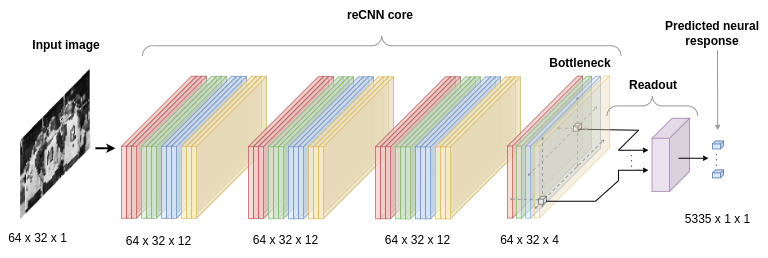
\includegraphics[width=145mm]{../img/architecture.png}
	\caption{A depiction of the proposed DNN architecture for Lurz et al. dataset \citep{lurz2021generalization}. An input image of resolution $64 \times 32$\,px is passed into a reCNN core with 4 layers equivariant to 4 rotations. The first three layers use 3 channels, which are reduced into a single channel in the bottleneck. Each color denotes a different orientation. The readout simultaneously learns the positions and orientations of all neurons, mapping them to positive real values corresponding to the neural responses. The numbers of layers, orientations and channels are chosen for the sake of clarity, not predictive performance. The optimal hyperparameters are described in Section \ref{best_lurz_section}.}
	\label{img_architecture}
\end{figure}

\section{Core: A rotation-equivariant CNN with a Bottleneck}

We implemented the above-described core and called it a \emph{reCNN bottleneck} as the last layer has a single channel for every rotation. Our approach consisted of adding a reCNN layer with one channel at the end of the core. Unfortunately, the Neuralpredictors library does not provide cores with a different number of channels in every layer, so the implementation was not straightforward. Firstly, we examined the implementation provided by Sinz lab, and with this knowledge, we appended the last layer.

As a nonlinear activation function, we use ELU. After each convolutional layer, a batch normalization layer follows. Input features are padded with zeros to maintain the same feature map size during the forward pass throughout the whole network.

Inspired by the paper from Lurz et al. \citep{lurz2021generalization}, we also allow the networks to use depth-separable convolutional layers \citep{chollet2017xception} in every layer after the first one. Whether to use them was based on the performance on the validation dataset.

Speaking of the core’s regularization, we utilized two forms of regularization, smoothness and group sparsity, both proposed by \citep{klindt2017neural}. Smoothness consists of the Laplacian of the convolution filters squared, that is:


\begin{equation}
L_{laplace} = \lambda_{laplace} \sum_{i, j, k, l} (W_{:, :, k, l} \star L)^2_{i, j},
\end{equation}

where $\lambda_{laplace}$ is a hyperparameter controlling the regularization strength, $W_{i, j, k, l}$ is the convolution kernel, $i$, $j$ are the spatial dimensions, and $k$ and $l$ are the input and output channels. Matrix $L$ is the Laplacian filter and is defined as follows:

\begin{equation}
L = \begin{bmatrix}
	0.5 & 1 & 0.5 \\
	1 & -6 & 1 \\
	0.5 & 1 & 0.5 \\
\end{bmatrix}
\end{equation}

Group sparsity regularization is defined as:

\begin{equation}
L_{group} = \lambda_{group} \sum_{i,j} \sqrt{\sum_{k, l} W^2_{i,j,k,l}},
\end{equation}

where $\lambda_{group}$ is the hyperparameter controlling the regularization’s importance, and $W_{i,j,k,l}$ is the convolution kernel described in the previous regularization term. Group sparsity forces the kernels to use a smaller number of features from the previous layer.


\section{Readout: A Three-Dimensional Gaussian Readout with a Cyclic Last Dimension}

Our second contribution is the readout. Similar to the readout proposed by Lurz et al. \citep{lurz2021generalization}, our readout layer estimates each neuron’s receptive field position in the core’s feature map, from which it subsequently fetches value and translates it into a neural response value. A three-dimensional extension of this readout is also available in the Neuralpredictors library. In addition to learning a neuron’s spatial position, it decides on one channel from which the value is yielded. 

We extended the third dimension to be periodic so that the strict interval mapping onto the orientation features does not impede the network’s training. Moreover, this cyclicity allows for a bilinear interpolation between the first and the last orientation features.

Regarding the implementation, whenever the readout reads a value from the third dimension out of the specified range $[-1, 1]$, the read position in this dimension is periodically shifted back into the interval $[-1, 1]$ and then mapped onto the feature map’s third dimension. The read value is obtained by bilinear interpolating the corresponding feature map’s units.

To impose periodicity on interval $[-1, 1]$, the position in the orientation dimension was adjusted in the following way:

\begin{equation}
o_{periodic} = ((o_{position} + 1) \text{ mod } 2) - 1
\end{equation}


This shifted the interval to $[0, 2]$, the modulo operation moved the position into the interval, and then we shifted the interval back to $[-1, 1]$. Concerning the first two dimensions, the positions to read the features from are clamped into the interval $[-1, 1]$. This is because retinotopy does not behave periodically; therefore, cyclicity is inappropriate in learning a neuron's position of its receptive field.

Although the above modification of the three-dimensional Gaussian readout samples values from features mapped to the interval $[-1, 1]$, it is not periodic yet. The orientation of value mapped to 1 does not correspond to the orientation of value in the feature map mapped to value $-1$. The first value corresponds to an orientation of 0\,degrees, and the last corresponds to $360\,(O - 1)/O $ degrees, where $O$ stands for the number of rotations. If we wanted to acquire value for orientation r such that $360\,(O - 1)/O < r < 360 = 0$ degrees, the readout would not be able to interpolate between $360\,(O - 1)/O$ and $360 = 0$ degrees. For example, if we had four possible orientations, the third dimension of the last reCNN core’s layer would have a size of 4, and the following degrees would be mapped to the values from $[-1, 1]$:



\begin{table}[H]\centering
	\begin{tabular}{ | c | c | } 
		\hline
		Value & Degree \\
		\hline
		-1 & 0 \\
		-$0.\overline{3}$ & 90 \\
		$0.\overline{3}$ & 180 \\
		1 & 270 \\ 
		\hline
	\end{tabular}
	\caption{Table of values and their corresponding degrees.}\label{tab001}
\end{table}


We copied all values from the feature map corresponding to an orientation of 0 degrees after the last layer to fix this issue. Consequently, the readout can properly fetch values from the core’s features employing bilinear interpolation even for values r such that $360\,(O - 1)/O< r < 360 = 0$ degrees. Sticking to numbers from above, we obtain this mapping of the interval $[-1, 1]$ to the orientation degrees:


\begin{table}[H]\centering
	\begin{tabular}{ | c | c | } 
		\hline
		Value & Degree \\
		\hline
		-1 & 0 \\
		
		-$0.5$ & 90 \\
		$0$ & 180 \\
		$0.5$ & 270 \\
		
		1 & 360 \\ 
		\hline
	\end{tabular}
	\caption{Fixed mapping of values to the corresponding degrees.}\label{tab002}
\end{table}


The interpolated value acquired by the readout is multiplied by a learned factor and shifted by a bias, which is initialized to a mean response of a particular neuron. Consequently, the value is passed into a Softplus activation function described in the chapter about feed-forward DNNs (Equation~\ref{softplus_equation}), yielding the final neuron’s response prediction. Since the readout is restricted to using just one position from the bottleneck, no regularization is imposed on the readout layer.


\section{Training Pipeline}

The process of finding the best model does not consist solely of a gradient-based algorithm for finding optimal model weights. In this section, we describe our training pipeline, including packaging the model, setting it up on remote servers, hyperparameter search, model training, and eventually evaluating and reusing the final trained model.

\subsection{Environment and Computational Resources}

To train the network, proper hardware with sufficient computational power is required. It is usually beneficial to containerize the solution into a software package that can be easily scaled and run on multiple machines.

We opted for Docker, a tool providing such containerization \citep{merkel2014docker}. We built a Docker image based on available Nvidia NGC containers\footnote{\url{https://catalog.ngc.nvidia.com/}} with installed PyTorch library and support for CUDA GPUs \citep{cuda} with other additional libraries, for instance, Neuralpredictors.

Due to a large number of parameters, the DNN’s training is computationally demanding. In our work, we harnessed resources provided by MetaCentrum\footnote{\url{https://www.metacentrum.cz/en/index.html}}. Because remote virtual machines obtained from a scheduling system on MetaCentrum use Singularity \citep{kurtzer2017singularity} instead of Docker, our Docker image had to be converted into an image compatible with Singularity. Fortunately, Singularity is prepared for this situation and made this conversion straightforward. Additionally, we developed multiple scripts simplifying the model’s deployment on the MetaCentrum infrastructure. 

\subsection{Hyperparameter Search}

In deep learning, finding the optimal hyperparameters is a crucial problem. The model’s author can either strictly set the hyperparameters according to previous experience, or some other algorithm is employed to search in a hyperparameter space, trying different solutions and using the best performing one on the validation set. During the hyperparameter search, it is favorable to track the experiments and model versions, visualize the results and later reproduce the models.


For these purposes, we utilized a machine learning tool Weights and Biases \citep{biewald2020experiment}, providing all the features mentioned above, which came in handy during the development. As regards the hyperparameter search, it can be done in multiple distinct ways. The most commonly used search techniques, which are also supported by Weights and Biases, are the following:
\begin{enumerate}
	\item Choose hyperparameter values randomly (random search).
	\item Given a finite hyperparameter space, try all possible hyperparameter values (grid search).
	\item Search for the optimal hyperparameters in a Bayesian fashion \citep{snoek2012practical}.
	
\end{enumerate}

We preferred the first and the last technique. The second option is not feasible in our case due to the infinite number of parameters to be set. Even discretizing the space of values that hyperparameters can take, due to the high dimensionality of it, covering it extensively is computationally unfeasible. 
At the beginning of our hyperparameter search, we employed a random search to get a gist of how the hyperparameter space behaves and weed out hyperparameters that do not yield a capable model.

Based on these empirical results, we narrowed the possible ranges of hyperparameter values to choose from, obtaining a smaller hyperparameter subspace. Consequently, we harnessed the Bayesian search to deliberately select the best hyperparameters. This technique prefers with some probability to select hyperparameters proven to perform well on the validation dataset based on the previous trials.

Weights and Biases provide a helpful feature for hyperparameter search called Sweeps. After a Sweep is initialized, virtual machines can connect to the Weights and Biases platform to acquire the next set of hyperparameters on which a network should be trained. Metrics, losses, and other valuable information are logged into the platform during training and can be consequently visualized in a web application provided by Weights and Biases.

\subsection{Control Model}

Only reporting the achieved values of the evaluation measures defined in Section~\ref{metrics_section} does not give the reader any gist of how using the bottleneck decreases the predictive performance. To give more context to our achieved performance, we developed and trained a model proposed in the paper from Lurz et al. \citep{lurz2021generalization}, mainly because they aim to create a core that generalizes well between different animals, making a perfect architecture for this comparison. In contrast with our model, Lurz and colleagues want to achieve the highest predictive performance possible with no restrictions. In contrast, our network has its computation strictly constrained by the bottleneck layer at the end of the reCNN core. It is, therefore, expected that our network will have much lower predictive performance. The question is, however, how much the performance drops.

For this reason, we compute the correlation fraction with respect to the control model. Specifically, this metric is obtained as the fraction of the correlation achieved by the bottleneck model over the correlation of the control model predictions. As regards the correlation used, we correlate each model’s predictions with the averaged response of the repeated trials. This result gives more information about the decrease in accuracy due to the bottleneck's presence and a readout that uses just a scalar value for a neuron’s response prediction.

This evaluation technique has, however, also an important drawback that needs to be taken into account. The control model’s quality influences the reported fraction of achieved performance. The worse the control model is, the better our bottleneck model seems to be. 









